%%% Sekce – Interaktivní mapa sedadel
%%%%% Wording: ✅
%%%%% Styling: ✅
%%%%% References: ✅
%%%%% Grammar: ✅
%%% --------------------------------------------------------------
\section{Interaktivní mapa sedadel}
\label{sec:implementace-seating}
Vývoj této webové aplikace zahrnoval několik klíčových prvků, z nichž každý představoval jedinečné výzvy a příležitosti.
Tyto prvky jsou základem funkčnosti aplikace a každý z nich hraje důležitou roli v celkovém uživatelském zážitku.

Prvním z těchto nepostradatelných prvků je interaktivní mapa sedadel.
Tento prvek umožňuje uživateli vizuálně procházet virtuální mapu sedadel v místnosti a vybrat si své preferované místo.
Mapa sedadel uživatelům poskytuje přehled o všech dostupných sedadlech, jejich kategoriích a stavech, čímž usnadňuje proces výběru sedadla a nákupu vstupenky.
Tato mapa je také zodpovědná za zobrazení informací o vstupenkách, které jsou přidruženy k vybraným sedadlům.

%%% Podsekce – Struktura
%%%%% Wording: ✅
%%%%% Styling: ✅
%%%%% References: ✅
%%%%% Grammar: ✅
%%% --------------------------------------------------------------
\begin{subsection}{Struktura}
    \label{subsec:implementace-seating-struktura}
    Struktura tohoto prvku je postavena na několika komponentách, které spolu harmonicky spolupracují.
    Primárními komponentami jsou:

    \begin{itemize}
        \item \texttt{SeatingMapProvider}
        \item \texttt{SeatingMap}
        \item \texttt{VirtualMap}
        \item \texttt{Seat}
        \item \texttt{SeatSheet}
    \end{itemize}

    \textbf{SeatingMapProvider} je nadřazená komponenta, která získává data z \ac{api} a zpřístupňuje je svým ostatním potomkům.
    Tato data zahrnují podrobnosti o místu konání, sedadlech, jejich stavech a vstupenkách.
    Více o získávání dat a jejich struktuře je popsáno v sekci~\ref{subsec:implementace-seating-data}.

    \textbf{SeatingMap} je komponenta, která zpracovává vstupní \ac{svg} data reprezentující mapu místa konání.
    Přebírá \ac{svg} data z \ac{api} a překládá je do formátu, který může být použit komponentou \texttt{VirtualMap}.

    \textbf{VirtualMap} je zodpovědná za přidání interaktivity do komponenty \texttt{SeatingMap}.
    Přidává ovládací funkce mapy, jako je posouvání, přibližování a oddalování, čímž poskytuje dynamický uživatelský zážitek.

    \textbf{Seat} a \textbf{SeatSheet} komponenty představují jednotlivá sedadla na mapě a podrobnosti zobrazené při jejich výběru.

    Souhra a struktura těchto komponent je znázorněna v zjednodušené ukázce kódu~\ref{listing:seating-map-structure} a na diagramu~\ref{fig:seating-map-structure}.

    \begin{listing}[H]
        \begin{minted}[breaklines]{html}
<SeatingMapProvider venue={venue}>
	{/* seating map */}
	<SeatingMap width={width} height={height}>
		{/* virtual map */}
		<VirtualMap minScaleFactor={1.1} maxScaleFactor={0.1}>
			{/* individual seats */}
			<Seat />
			<Seat />
			<Seat />
			{/* + any other svg elements */}
		</VirtualMap>

		{/* seat sheet detail */}
		<Sheet>
			<Sheet.Header />
			<Sheet.Body>
				<SeatSheet />
			</Sheet.Body>
		</Sheet>
	</SeatingMap>
</SeatingMapProvider>
        \end{minted}
        \caption{Struktura komponent mapy sedadel}
        \label{listing:seating-map-structure}
    \end{listing}

    \begin{figure}[H]
        \centering
        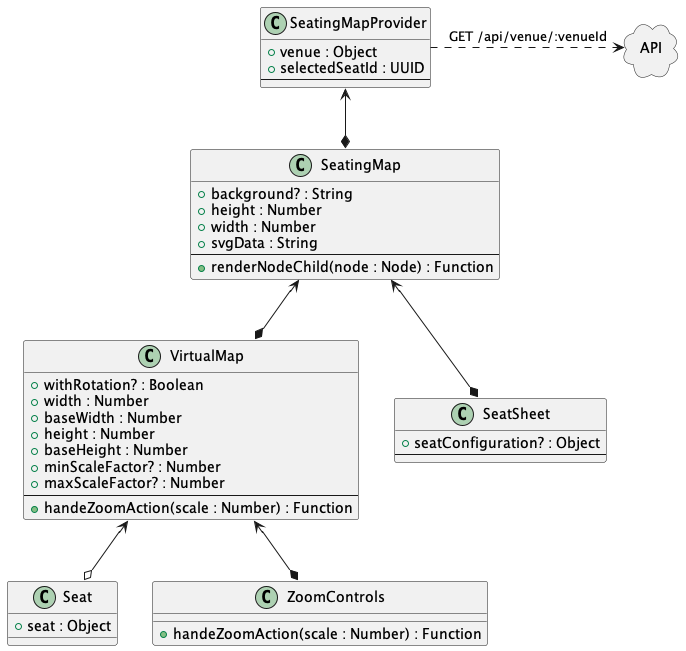
\includegraphics[width=\textwidth]{\FIGDIR/diagrams/seating-map}
        \caption{Diagram komponent mapy sedadel}
        \label{fig:seating-map-structure}
    \end{figure}
\end{subsection}

%%% Podsekce – Získávání a správa dat
%%%%% Wording: ✅
%%%%% Styling: ✅
%%%%% References: ✅
%%%%% Grammar: ✅
%%% --------------------------------------------------------------
\begin{subsection}{Získávání a správa dat}
    \label{subsec:implementace-seating-data}
    Proces získávání a správy dat začíná komponentou \texttt{SeatingMapProvider}.
    Tato komponenta vytvoří požadavek na \ac{api}, aby získala data týkající se uspořádání sedadel daného místa konání.

    Odpověď \ac{api} zahrnuje podrobnou \ac{svg} reprezentaci uspořádání sedadel a jejich jednotlivá data.
    Každé sedadlo obsahuje informace o jeho řadě, místě, plném názvu, dostupné kapacitě a přidružených vstupenkách a kategoriích.
    Každá vstupenka obsahuje informace o jejím id, názvu, volitelném popisu, ceně a kategoriích.
    Podrobná struktura dat je znázorněna v ukázce kódu~\ref{listing:venue-api-schema}.

    \begin{listing}[H]
        \begin{minted}[breaklines]{typescript}
/**
 * Venue API response schema
 * @export
 */
export const venueApiSchema = z.object({
	venueId: z.string().uuid(),
	name: z.string(),
	/** seating drawing (SVG) */
	drawing: z.string(),
	/** venue seat data */
	seats: z.array(
		z.object({
			seatId: z.string().uuid(),
			row: z.string(),
			place: z.number(),
			fullName: z.string(),
			capacityLeft: z.number(),
			tickets: z.array(z.string().uuid()),
			categoryId: z.string().uuid(),
		}),
	),
	/** venue ticket data */
	tickets: z.array(
		z.object({
			ticketId: z.string().uuid(),
			name: z.string(),
			description: z.string().optional(),
			price: z.number().int(),
			categories: z.array(
				z.object({
					categoryId: z.string().uuid(),
					price: z.number().int(),
				}),
			),
		}),
	),
	/** venue ticket categories */
	categories: z.array(
		z.object({
			categoryId: z.string().uuid(),
			name: z.string(),
			description: z.string().optional(),
			color: z.string(),
		}),
	),
});
        \end{minted}
        \caption{Struktura odpovědi \ac{api} obsahující data o uspořádání sedadel}
        \label{listing:venue-api-schema}
    \end{listing}

    Po získání těchto dat komponenta \texttt{SeatingMapProvider} tato data zpracuje do použitelnějšího formátu.
    Toto zpracování zahrnuje oddělení sedadel, vstupenek a kategorií do vlastních struktur, vytvářející hierarchii, která zjednodušuje přístup k datům pro následující komponenty.

    Tento zpracovaný formát je pak ostatním komponentám zpřístupněn pomocí \foreign{Context API}\footnote{\url{https://react.dev/learn/passing-data-deeply-with-context}}, což poskytuje pohodlný způsob, jak k nim přistupovat nezávisle na jejich umístění ve stromu komponent.
\end{subsection}

%%% Podsekce – Parsování SVG a mapování sedadel
%%%%% Wording: ✅
%%%%% Styling: ✅
%%%%% References: ✅
%%%%% Grammar: ✅
%%% --------------------------------------------------------------
\begin{subsection}{Parsování SVG a mapování sedadel}
    \label{subsec:implementace-seating-svg}
    \texttt{SeatingMap} komponenta je zodpovědná za parsování příchozích \ac{svg} dat a jejich překlad do formátu, který může být použit komponentou \texttt{VirtualMap}.

    Příchozí \ac{svg} data mají specifickou strukturu, kde \mintinline{html}{<g>} elementy představují skupiny sedadel, a jsou identifikovány pomocí id atributu ve formátu \texttt{"seats:xxx"}, kde \texttt{xxx} je identifikátor konkrétní skupiny sedadel.
    Jednotlivá sedadla v rámci těchto skupin jsou reprezentována \mintinline{html}{<circle>} či \mintinline{html}{<rect>} elementy, identifikovanými jejich jedinečnými id ve formě \texttt{"seat:row+place"}, kde \texttt{row} je řada sedadla a \texttt{place} je číslo místa v rámci řady.
    Zjednodušené znázornění této struktury je vyobrazeno v ukázce kódu~\ref{listing:seating-svg-structure}.

    \begin{listing}[H]
        \begin{minted}{xml}
<svg width="1287" height="1115" viewBox="0 0 1287 1115" fill="#F2F4F7" xmlns="http://www.w3.org/2000/svg">
    <!-- seats -->
    <g id="seats:back">
        <!-- seat H+1 -->
        <circle id="seat:H+1" cx="48" cy="785" r="50" fill="#D0D5DD"/>
        <!-- seat I+1 -->
        <circle id="seat:I+1" cx="48" cy="805" r="50" fill="#D0D5DD"/>
        <!-- ... -->
    </g>
    <g id="seats:right">
        <!-- ... -->
    </g>
    <g id="seats:left">
        <!-- ... -->
    </g>
    <g id="seats:center">
        <!-- ... -->
    </g>
    <!-- details -->
    <g id="details:patio">
        <!-- ... -->
    </g>
    <!-- ... -->
</svg>
        \end{minted}
        \caption{Ukázka struktury \ac{svg} dat}
        \label{listing:seating-svg-structure}
    \end{listing}

    Parsování těchto dat probíhá za pomoci knihovny \texttt{svg-parser}\footnote{\url{https://www.npmjs.com/package/svg-parser}} a výsledkem je upravená struktura, kde je každé sedadlo (reprezentované \mintinline{html}{<circle>} či \mintinline{html}{<rect>} elementem) nahrazeno dedikovanou komponentou \mintinline{html}{<Seat />}, jejíž funkčnost je dále rozepsána v sekci~\ref{subsec:implementace-seating-seat}.
\end{subsection}

%%% Podsekce – Interaktivita s VirtualMap
%%%%% Wording: ✅
%%%%% Styling: ✅
%%%%% References: ✅
%%%%% Grammar: ✅
%%% --------------------------------------------------------------
\begin{subsection}{Interaktivita s VirtualMap}
    \label{subsec:implementace-seating-virtualmap}
    Komponenta \texttt{VirtualMap} přidává interaktivitu do mapy sedadel.
    Tato komponenta obaluje komponentu \texttt{SeatingMap}, přebírající parsované a namapované \ac{svg} elementy jako své potomky, a zajišťuje všechny interakce s mapou sedadel.

    Tato komponenta využívá knihovny \texttt{react-spring}\footnote{\url{https://www.npmjs.com/package/react-spring}} a \texttt{use-gesture}\footnote{\url{https://www.npmjs.com/package/@use-gesture/react}} k zajištění plynulé a responzivní animace pro gesta \foreign{pan}\footnote{\foreign{Pan} je gesto, které umožňuje uživateli posunout obsah v rámci omezeného prostoru.} a \foreign{pinch}\footnote{\foreign{Pinch} je gesto, které umožňuje uživateli přiblížit nebo oddálit obsah.
    }, poskytující dynamický a plynulý uživatelský zážitek.

    Komponenta \texttt{VirtualMap} také zajišťuje správu stavu mapy, sledováním změn, jako je úroveň \foreign{zoom}\footnote{\foreign{Zoom} je úroveň přiblížení nebo oddálení obsahu.} a posunutí.
    Tato správa stavu zajišťuje především konzistentní uživatelský zážitek při manipulaci mapy uživatelem.
\end{subsection}

%%% Podsekce – Výběr sedadla a správa vstupenek
%%%%% Wording: ✅
%%%%% Styling: ✅
%%%%% References: ✅
%%%%% Grammar: ✅
%%% --------------------------------------------------------------
\begin{subsection}{Výběr sedadla a správa vstupenek}
    \label{subsec:implementace-seating-seat}
    Komponenty \texttt{Seat} a \texttt{SeatSheet} jsou zodpovědné za výběr sedadla a správu komunikace s nákupním košíkem.

    Komponenta \texttt{Seat} reprezentuje jednotlivá sedadla na mapě a spravuje všechna jeho příslušná data, jako je jeho dostupnost a aktuální stav.
    Kliknutím na jakékoliv sedadlo se vyvolá akce zvolení sedadla, která spustí otevření komponenty \texttt{SeatSheet}, která poskytuje uživatelsky přívětivé rozhraní pro zobrazení informací o daném sedadle a výběr z možných vstupenek.

    \begin{figure}[h]
        \centering
        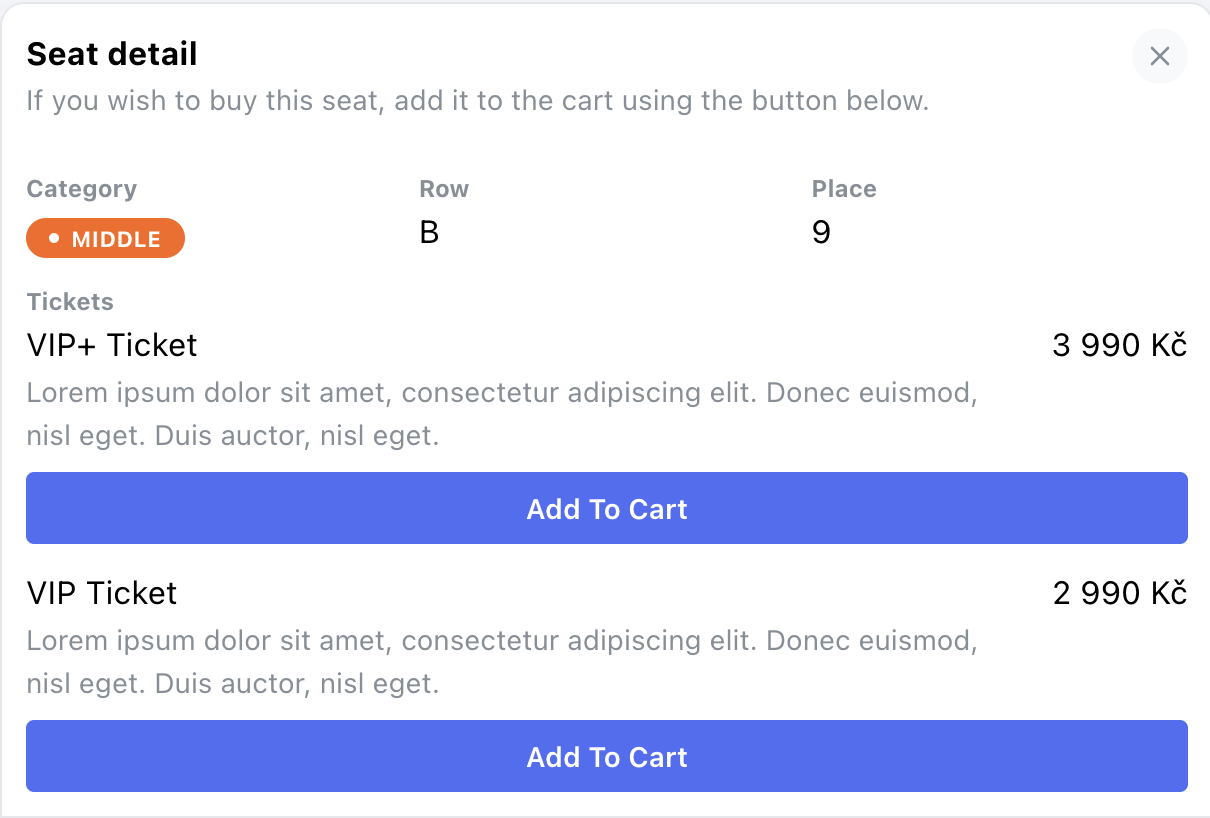
\includegraphics[width=0.75\textwidth]{\FIGDIR/seating-map-seat-sheet}
        \caption{Snímek obrazovky komponenty \texttt{SeatSheet}}
        \label{fig:seating-map-seats-sheet}
    \end{figure}

    Na obrázku~\ref{fig:seating-map-seats-sheet} je zobrazena komponenta \texttt{SeatingSheet} s detaily vybraného sedadla, včetně jeho kategorie, řady, místa a dostupných vstupenek.

    Vstupenky jsou vázány na kategorii sedadla a kategorie může mít několik příslušných vstupenek.
    Cena vstupenky je poté definována kombinací její kategorie a vybraného sedadla.

    Uživatel může přidat vybranou vstupenku do svého košíku přímo z rozhraní komponenty \texttt{SeatSheet}.
    Pokud je v košíku již vstupenka pro vybrané sedadlo, může uživatel vybrat, zda chce vstupenku vyměnit nebo ji z košíku odebrat.
    Všechny tyto změny se okamžitě promítají v uživatelském rozhraní a poskytují tak uživateli zpětnou vazbu v reálném čase.

    \begin{figure}[h]
        \centering
        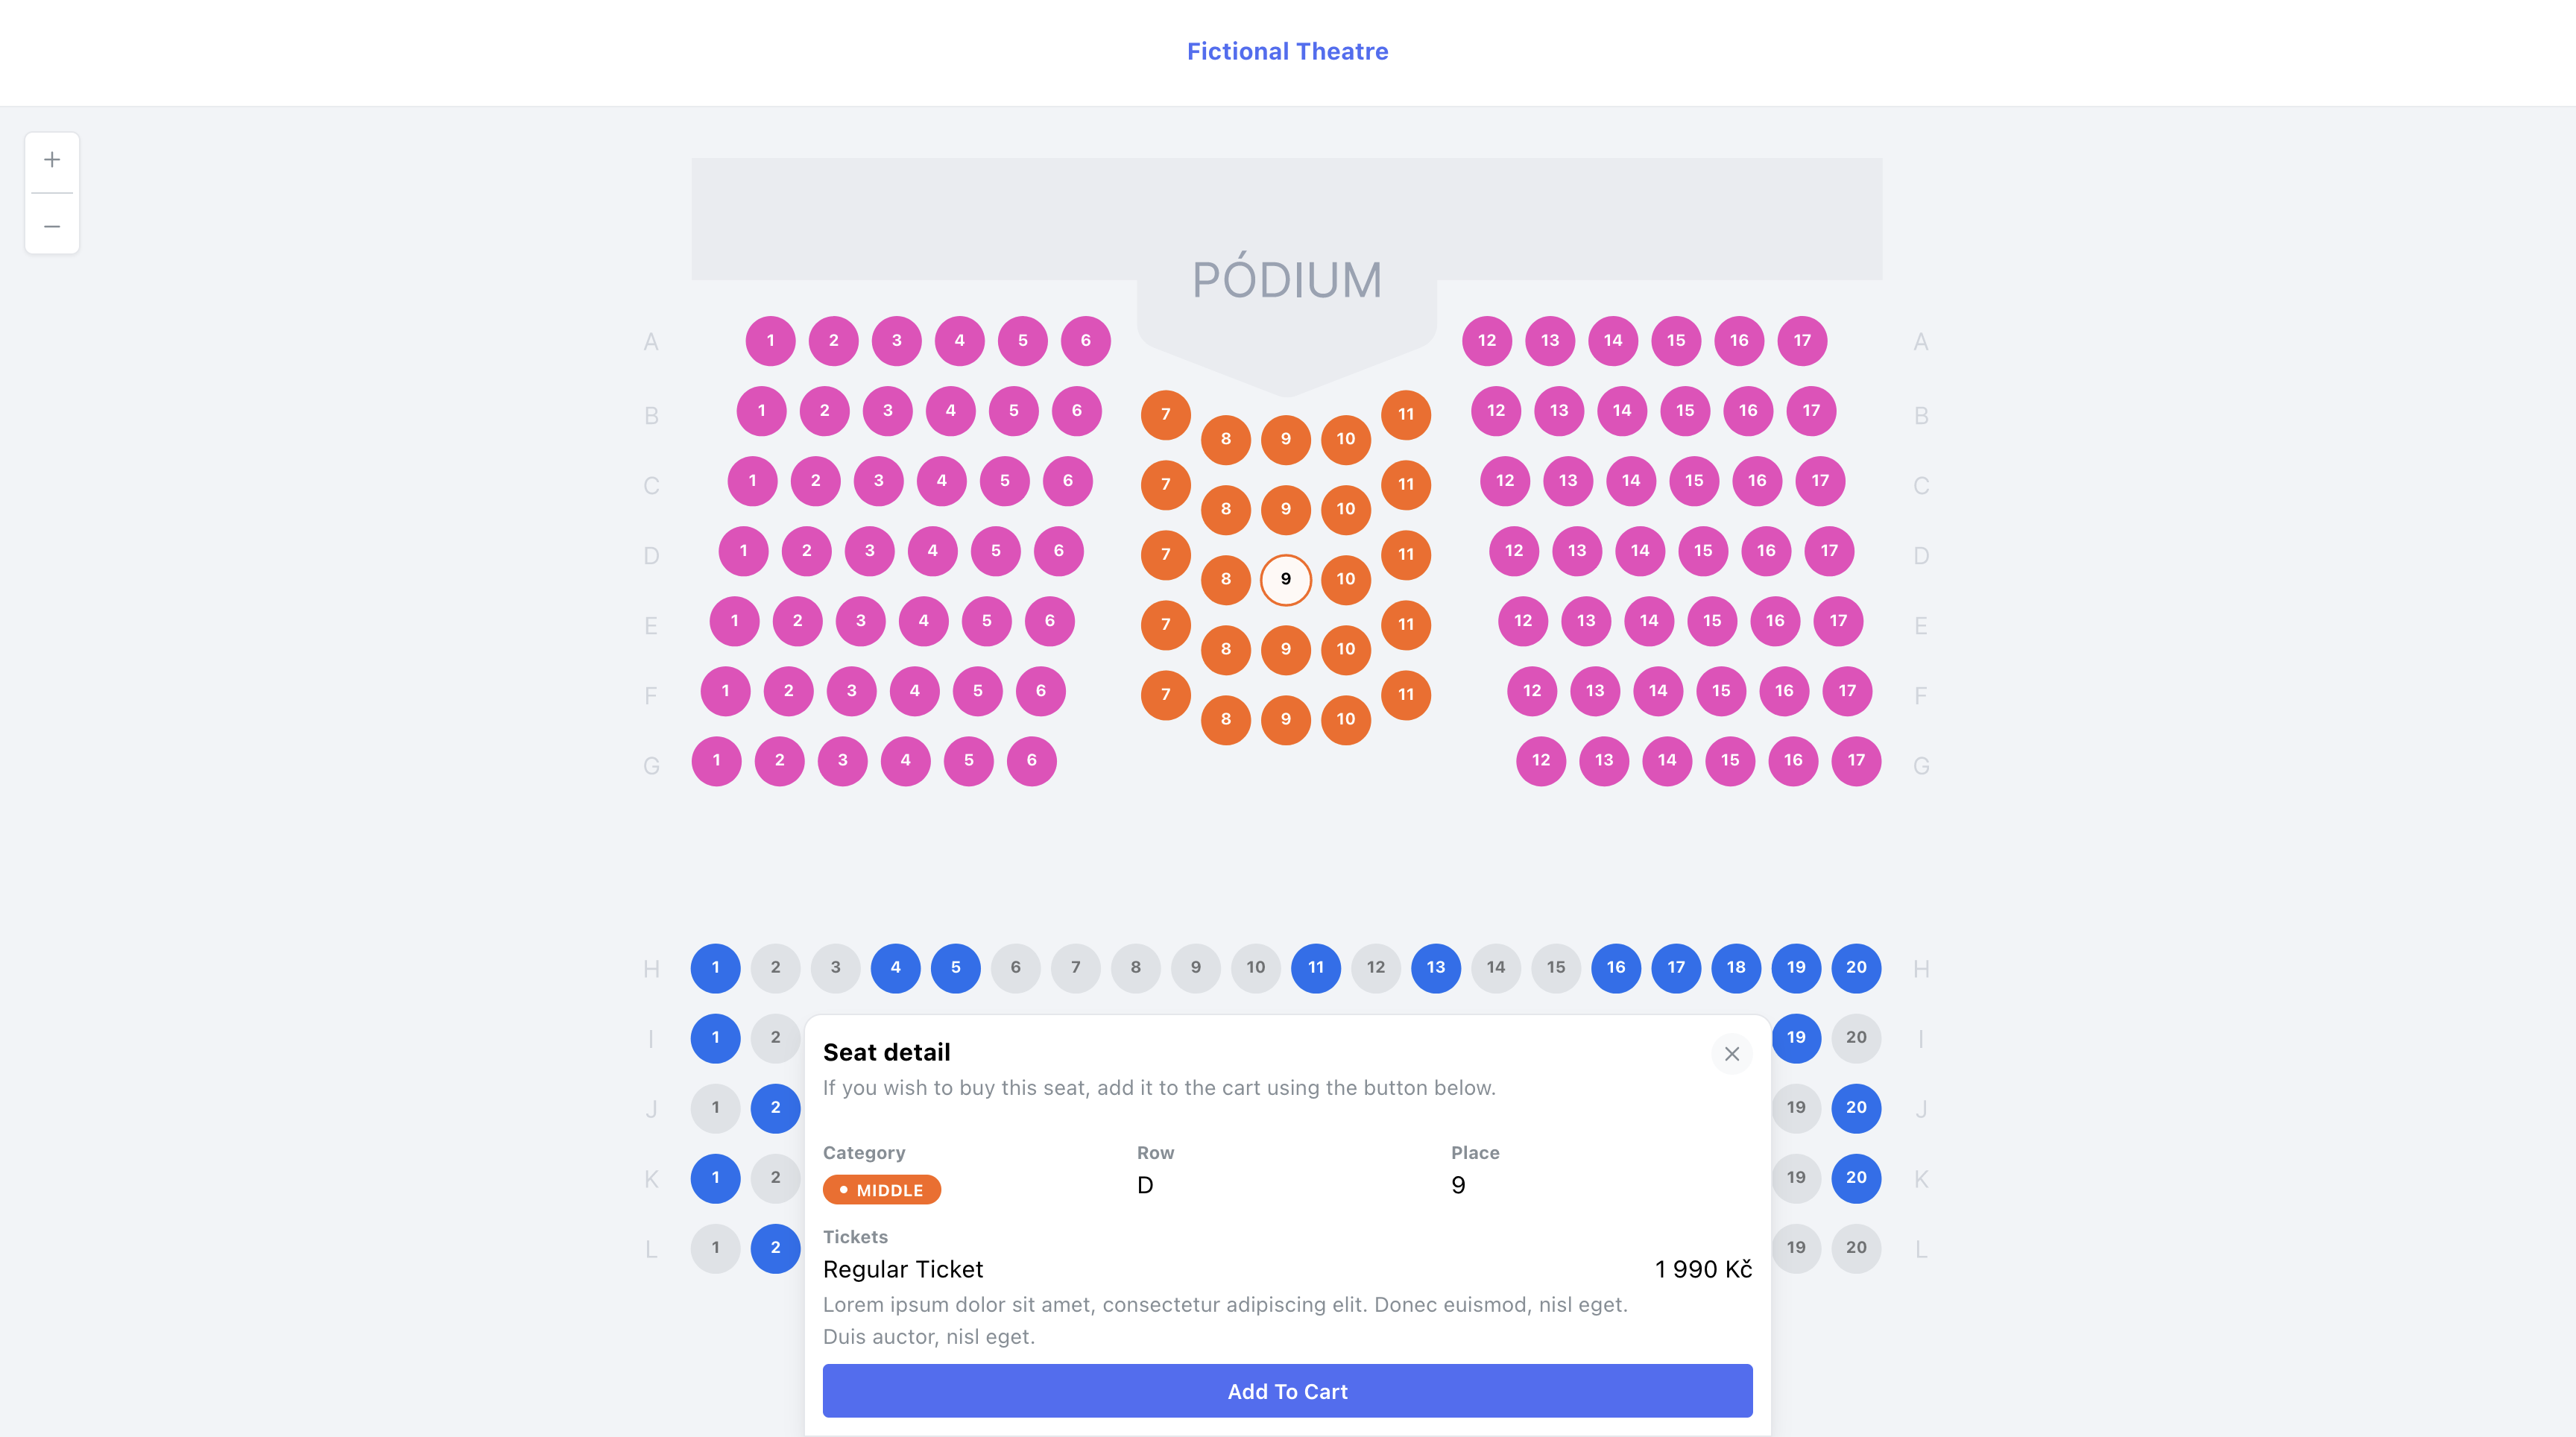
\includegraphics[width=\textwidth]{\FIGDIR/seating-map-seat}
        \caption{Snímek obrazovky interaktivní mapy sedadel}
        \label{fig:seating-map-seat}
    \end{figure}

    Obrázek~\ref{fig:seating-map-seat} zobrazuje výsledný produkt, ilustrující uživatelsky přívětivé rozhraní a dynamickou mapu sedadel.
    Kombinace výše uvedených komponent umožňuje snadnou navigaci sedadel místa konání, okamžitý přístup k informacím o vstupenkách a přehlednou správu vstupenek zajišťující efektivní nákupní proces.
\end{subsection}
